%%%%%%%%%%%%%%%%%%%%%%%%%%%%%%%%%%%%%%%%%%%%%%%%%%%%%%%%%%%%%%%%%%%%%%%%%%%%%%%%
%2345678901234567890123456789012345678901234567890123456789012345678901234567890
%        1         2         3         4         5         6         7         8

\documentclass{TeXstyles/DARS/svmult}  % Comment this line out
                                                          % if you need a4paper
%\documentclass[a4paper, 10pt, conference]{ieeeconf}      % Use this line for a4
                                                          % paper

%\IEEEoverridecommandlockouts                              % This command is only
                                                          % needed if you want to
                                                          % use the \thanks command
%\overrideIEEEmargins
% See the \addtolength command later in the file to balance the column lengths
% on the last page of the document

% Usual setup packages
\usepackage{times}
\usepackage[utf8]{inputenc} % set input encoding (not needed with XeLaTeX)
\usepackage{geometry} % to change the page dimensions
\usepackage{graphicx} % General page control package
%\usepackage[compact]{titlesec} % For compact title
\usepackage{listings} % For including source code with highlighting
\usepackage{subfiles} % For better multiple file per paper handling
\usepackage{hyperref} % For better hyper-link integration

% Packages for verbatim text blocks
\usepackage{alltt} % Package for including math in verbatim text
\usepackage{fancyvrb}

% Packages for math symbols and other mathey things
\usepackage{amsmath}
\usepackage{amsfonts}
\usepackage{amssymb}

% Packages for including pseudo-code
\usepackage{algorithmicx}
\usepackage{algorithm}
\usepackage{algpseudocode}

% Packages that handle lists
\usepackage{enumerate} % For reduced enumeration spacing
\usepackage{mdwlist} % Better control of lists

% Packages that handle tables, figures and other floats
\usepackage{tabularx}
\usepackage{multirow}
%\usepackage{titling}
\usepackage{float} % To make floats movable
\usepackage[font=scriptsize,labelfont=bf]{caption}
\usepackage[font=scriptsize,labelfont=bf]{subcaption}
\usepackage[table]{xcolor}

% Packages for drawing graphs, FSMs, etc.
\usepackage{pgf}
\usepackage{tikz}
\usetikzlibrary{shapes,arrows,calc,fit,positioning,shapes.symbols,shapes.callouts,patterns,automata}

% Remove red boxes around refs
\hypersetup{
    colorlinks,
    citecolor=black,
    filecolor=black,
    linkcolor=black,
    urlcolor=blue
}

% Nice Little macro for adding a comment box. Include incrementing comment numbers.
\newcounter{comcount}
\setcounter{comcount}{0}
\newcommand{\mycomment}[1]
{
\refstepcounter{comcount}
\smallskip\noindent\fbox{\parbox{\linewidth}{\emph{Comment \arabic{comcount}} : \small{#1}}} 
}

\newcommand{\sig}{\mathcal{S}}
\newcommand{\ceil}[1]{\lceil#1\rceil}


\title*{A Response Threshold Sigmoid Function Model for Swarm Robot Collaboration}

\author{Anshul Kanakia and Nikolaus Correll}

\institute{Anshul Kanakia \at University of Colorado, Boulder\\ Dept. of Computer Science\\ \email{anshul.kanakia@colorado.edu}
\and Nikolaus Correll \at University of Colorado, Boulder\\ Dept. of Computer Science\\ \email{nikolaus.correll@colorado.edu}}

\begin{document}
\maketitle
%\thispagestyle{empty}
%\pagestyle{empty}


%%%%%%%%%%%%%%%%%%%%%%%%%%%%%%%%%%%%%%%%%%%%%%%%%%%%%%%%%%%%%%%%%%%%%%%%%%%%%%%%
\abstract{
We present a multi-agent collaboration algorithm to recruit an approximate number of individually simple robots. We propose a sigmoid response threshold function motivated by task allocation in social insects, and describe macro-level models backed by micro-level simulations to predict the resulting team sizes and their variance. We show that the slope of the response threshold function can be used to control the variance of group size, allowing agents to trade off deterministic team size with coordination speed, making the proposed mechanism applicable to a variety of applications.}
%%%%%%%%%%%%%%%%%%%%%%%%%%%%%%%%%%%%%%%%%%%%%%%%%%%%%%%%%%%%%%%%%%%%%%%%%%%%%%%%



%%%%%%%%%%%%%%%%%%%%%%%%%%%%%%%%%%%%%%%%%%%%%%%%%%%%%%%%%%%%%%%%%%%%%%%%%%%%%%%%
\section{Introduction}
We propose a probabilistic, threshold based multi agent collaboration algorithm and analysis to recruit an \emph{approximate} number robots. Recruiting a number of robots to collaboratively solve a task is a canonical problem in robotics \cite{Gerkey2004}. Formally introduced in the stick-pulling experiment as described by Martinoli et al.~\cite{Martinoli2004, Martinoli1995} to recruit exactly two robots to collaboratively pull a stick out of the ground, Lerman et al.~\cite{Lerman2001} have extended this model to larger teams of constant size. In each case the result of collaboration is binary, success or failure, based on whether an exact number of robots are present at the collaboration site or not. %

We wish to extend the stick pulling model of constant group sizes of robots to include a more general case of collaboration tasks that involve only approximate numbers of robots for successful collaboration. Examples of such tasks include collective transport \cite{sugawara2012}, pattern recognition \cite{beni1993swarm}, real-time mapping of oil spills \cite{beni2005swarm}, determining coverage area of forest fires \cite{krishnanand2006glowworm}, aerial swarm surveillance \cite{dantu2012comparison}, and many others that require a subset of a swarm to coalesce to tackle a task collaboratively. It is important to note that we do not study any particular task in detail but rather, outline a general approach to modeling scenarios with the aforementioned properties. In such cases, so long as we have at least one robot, the task may be accomplished with varying degrees of success. Here, tuning the permissible variance allows to tune the likelihood with which such worst case collaborations happen. Formally understanding the dynamics of the underlying coordination mechanisms allows the designer not only to predict performance, but also to optimize a swarming system \cite{Correll2008}.  

The proposed algorithm and model is inspired from task allocation in biological systems such as ant colonies \cite{Bonabeau1999,Krieger2000}. We employ the use of a response threshold sigmoid function that probabilistically triggers the beginning of a collaboration step between robots at the same collaboration site. We study this approach via macroscopic models and microscopic simulations.
The sigmoid function used in our model is commonly referred to as the \emph{Logistic} function and has control parameters that allow us to alter its offset and slope. We study the effects that changing these parameters has on the system-wide behavior of the robot swarm. We also draw comparisons between this collaboration model and similar models used by Lerman et al. for the \emph{n}-robot stick pulling experiment \cite{Lerman2001} and discuss situations where it is beneficial to use one model over the other.

The rest of the paper is organized as follows. Section \ref{sec:expsetup} introduces the task allocation algorithm that we will be studying throughout the course of the paper.
Section \ref{sec:macromodel} provides a mathematical basis for the threshold based collaboration model and attempts to explain how the voting strategy being employed affects group sizes and their variance.
Section \ref{sec:micromodel} provides an explanation of the agent level controller in the system. This section further outlines the experimental setup being used to run simulations and the important parameters of the system. 
We compare collaboration rates of our model with the constant group size model introduced by Lerman et al.~\cite{Lerman2001} using micro-level Gillespie simulation in Section \ref{sec:micromodel}, showing that the dynamics are comparable for similar team sizes, yet allow us to tune the variance of the resulting group size.  
Finally, Sections \ref{sec:discussion} and \ref{sec:conclusion} provide discussion of the drawbacks and limitations of the proposed model and scenarios where it could fail as well as discussing possible avenues for future work.

\subsection{Related work}
Task allocation is a canonical problem in multi-robot systems \cite{Gerkey2004}. Whereas capable robots might be able to approximate optimal task allocation, e.g., using market-based approaches \cite{amstutz2008distributed,vig2007coalition} or using  leader-follower coalition algorithms \cite{Chen2011}, probabilistic algorithms are of particular interest for swarm robotics with individually simple controllers \cite{dantu2012comparison}. To recruit an exact number of robots to a particular task has been extensively studied at the hands of the ``Stick Pulling'' experiment \cite{Lerman2001,Martinoli2004}, whereas to distribute a swarm of robots across a discrete number of sites/tasks with a specific desired distribution has been studied in \cite{Berman2009,Correll2008}. The proposed algorithm extends upon the first group of work, and we show how the proposed stochastic task allocation algorithm reduces to \cite{Lerman2001,Martinoli2004} when using appropriate parameters.  Mather \cite{mather2010towards} instead presents a stochastic approach that is a hybrid between the work in \cite{Berman2009} and \cite{Martinoli2004}, allowing allocation to tasks requiring a varying number of robots.
While a response threshold function can also be applied to the swarm distribution problem, this problem is complementary to the problem of recruiting a team of a specific size. 



%%%%%%%%%%%%%%%%%%%%%%%%%%%%%%%%%%%%%%%%%%%%%%%%%%%%%%%%%%%%%%%%%%%%%%%%%%%%%%%%
\section{Response threshold-based task allocation}\label{sec:expsetup}
\begin{figure}[!htb]
\centering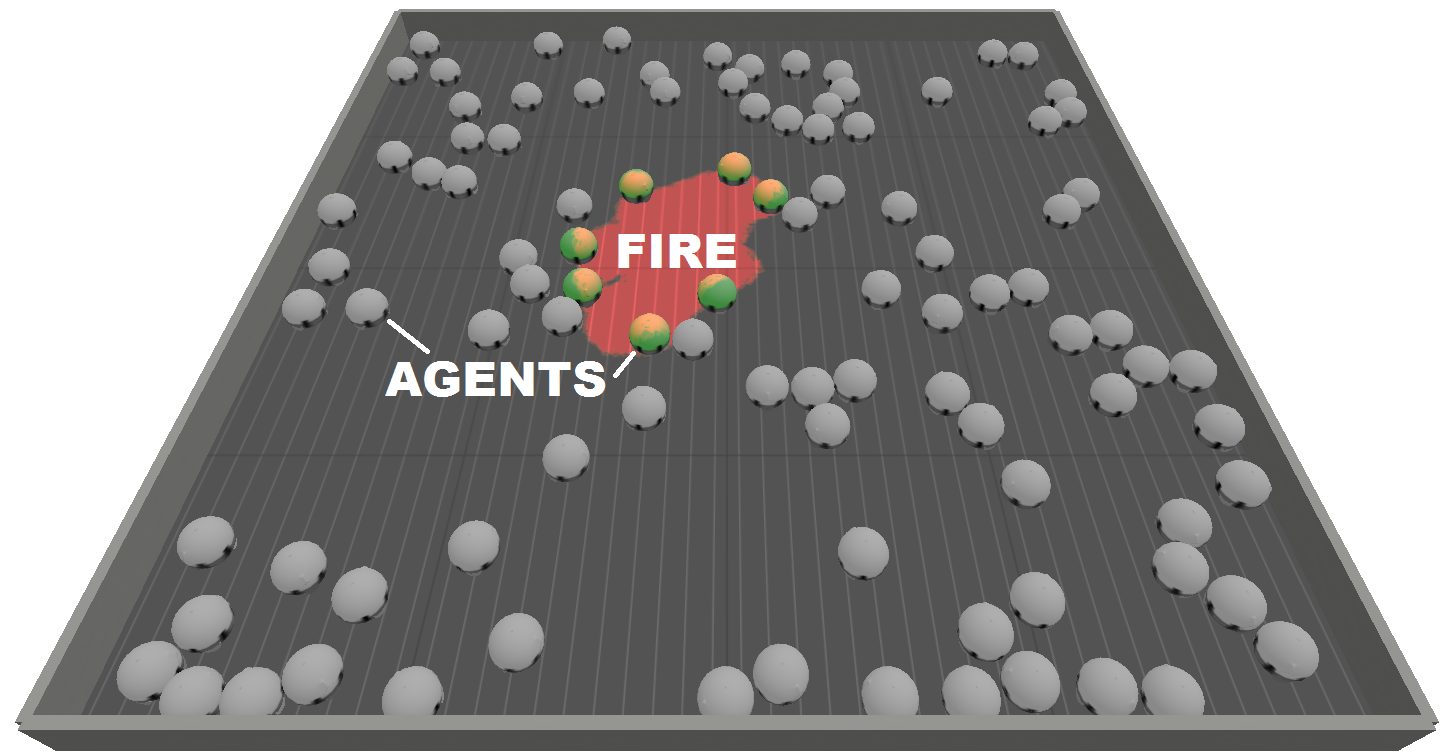
\includegraphics[width=7cm]{figures/setup.png}
\caption{A visual representation of the collaboration experiment being studied.}\label{fig:setup}
\end{figure}
We consider a generic collaboration task with $m$ uniformly distributed collaboration sites within a flat arena with area, $A$. A swarm of individually simple robots is deployed within the arena, also uniformly and at random as shown in Fig.~\ref{fig:setup}. The number of robots being used per experiment varies, as we discuss results for a number of different scenarios. Collaboration sites in the arena can be of various sizes and configurations.

Each individual agent is capable of locomotion and local sensing. The agents do not require global positioning and no centralized controller exists, but we assume each agent to be capable of local omnidirectional communication with other agents within its communication range. The agents are also capable of sensing the boundary of a collaboration site---we assume that sites have easily distinguishable boundary regions for the purposes of the model studied in this paper.

The objective of each agent in the robot swarm is to find a collaboration site in the arena and perform a collective task with other agents at that site. The precise details of the collective task are not important for the purpose of understanding the coordination mechanism. We assume the actual collective task takes each agent a probabilistic, finite amount of time to complete. Once collaboration is complete, the robot detaches itself from its current site and returns to searching for more sites in the arena. 

\begin{figure*}[!htb]
\centering\begin{subfigure}{.5\textwidth}
\centering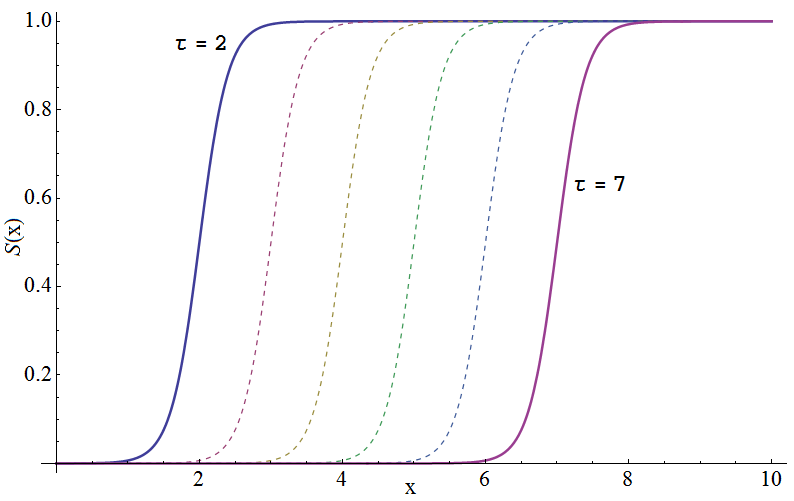
\includegraphics[width=7.5cm]{figures/sigmoid2.png}
\caption{Changing $\tau$ offsets the curve along the $x$ axis, allowing to set the desired mean team size.}\label{}
\end{subfigure}~
\centering\begin{subfigure}{.5\textwidth}
\centering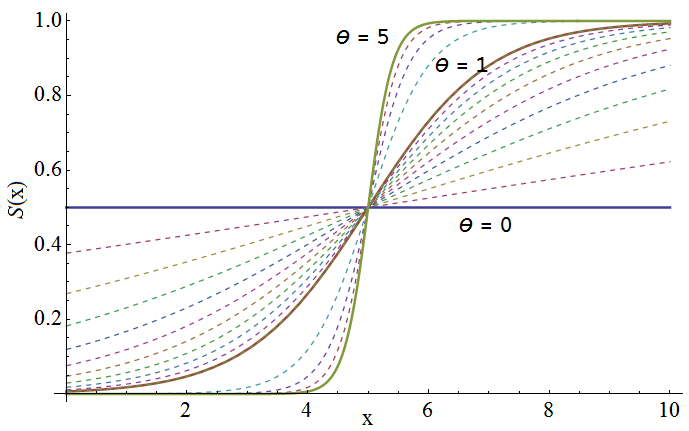
\includegraphics[width=7.5cm]{figures/sigmoid1.png}
\caption{Changing $\theta$ changes the slope at the point $x^* = \tau$, $\sig(x^*) = 0.5$, allowing to control the team's variance.}\label{}
\end{subfigure}~
\caption{Sigmoidal response threshold function and its parameters.}\label{fig:sig}
\end{figure*}

It is perfectly reasonable to assume that agents arrive at the same collaboration site after having just completed a task there (possibly unsuccessfully) but will now be part of a new collaboration group. Each agent individually decides whether or not to collaborate at a given time step, while waiting at a collaboration site. If the majority of agents currently at a collaboration site decides to collaborate, then the entire population is recruited for the task and thus a collective consensus is reached using a majority voting scheme. Here, we consider a ``majority'' to mean exactly half or more of a given population. An individual agent's willingness to collaborate is a stochastic term governed by a sigmoid based threshold function, that takes as input the number of agents $x$ currently at the same collaboration site as seen/sensed by each individual agent:
\begin{equation}
	\sig(x) = \frac{1}{1+e^{\theta(\tau - x)}}\label{eq:sig}
\end{equation}
The parameter $\theta$ controls the slope of the sigmoid function, while $\tau$ controls its offset along the $x$ axis, as seen in Fig.~\ref{fig:sig}. For the purpose of task allocation, $\tau$ is the average desired group size at which an agent group should collaborate. The input, $x$, is the estimated group size currently at the same collaboration site as the agent. Each agent is independently responsible for estimating the group size at a given time either by direct sensing or by communication. In practice,  this involves building a list of unique identifiers of the agents sharing its collaboration site. This algorithm, followed by each individual agent in the system, is provided in Algorithm \ref{alg:sigalg}.

Note that the proposed response threshold function is different from \cite{Bonabeau1999}, who uses high-order polynomials. While these functions work well in regimes with moderate slope, they create numerical problems when approximating unit-step-like responses such as those (implicitly) used in \cite{Lerman2001}. We particularly chose the logistic function from the large class of sigmoid functions due to the intuitive nature of the parameters $\tau$ and $\theta$. 

\begin{algorithm}
\caption{Task allocation algorithm for an individual agent using the sigmoid threshold function}
\label{alg:sigalg}
\begin{algorithmic}
	\Function{Task\_Allocation}{$\theta$, $\tau$}
	\State $estimate \gets$ discover\_group\_size()
	\State $decision \gets$ run\_sigmoid($estimate$, $\theta$, $\tau$)
	\State communicate\_decision($decision$)
	\State $decisions[] \gets$ gather\_decisions()
	\State $result \gets$ Count($decisions[]$, $true$) \Comment{Count() Returns the number of successes in the decisions}
	\If{$result \geq (estimate / 2)$}
		\State Collaborate()
		\State \Return
	\Else
		\State Task\_Allocation($\theta$, $\tau$)
	\EndIf
	\EndFunction
\end{algorithmic} 
\end{algorithm}





%%%%%%%%%%%%%%%%%%%%%%%%%%%%%%%%%%%%%%%%%%%%%%%%%%%%%%%%%%%%%%%%%%%%%%%%%%%%%%%%
\section{Macroscopic analysis}\label{sec:macromodel}
In this section we study how the proposed algorithm leads to the desired behavior, an average group size of $\tau$ with variance proportional to $\theta$ on macroscopic level. 

\subsection{A general model of probabilistic task allocation}
Equation \eqref{eq:sig} is a cumulative probability density function approaching $1.0$ as the number of agents approaches infinity, that is $\lim_{x \to \infty}\sig(x)=1$. For $\theta \to \infty$, equation \eqref{eq:sig} approximates the unit step, except for the special case $x=\tau$:
\begin{equation}
\lim_{\theta \to \infty} \frac{1}{1+e^{\theta(\tau-x)}}=
\left\{
\begin{array}{cc}
 x>\tau & 1\\
 x=\tau	 & \frac{1}{2}\\
 x<\tau & 0
\end{array}
\right.
\end{equation}
The discontinuity at $x=\tau$ is the rational for having collaboration to include half or more of the agents to decide to collaborate. Including the mid-point makes the agents behave like they are using a unit-step function in the case of $\theta \to \infty$. The proposed model is therefore a generalization of the ``stick-pulling'' task allocation model with deterministic team size \cite{Lerman2001}, allowing us to tune the variance of the resulting group sizes. 

\subsection{From individual choices to team-level collaboration}
Assuming the agents to be loosely synchronized, e.g., by considering decisions within a finite window of time, determining a majority vote corresponds to a Bernoulli trial with each agent flipping a biased coin---the bias being computed using the sigmoid function---to decide whether or not to collaborate in the next time step. The probability that exactly $k$ agents collaborate from a population of $n$ agents at a collaboration site is given by the probability mass function (pmf) of a Binomial distribution.
\begin{equation}
	B(n, k) = \binom{n}{k}\sig(n)^{k}\left(1 - \sig(n)\right)^{n - k}\label{eq:binomial}
\end{equation}

Since we care about the case when half or more of the agents (${n/2}$) decide to collaborate, the probability $P(n)$ that half or more agents in a group of $n$ collaborate is the cumulative probability of the above pmf from $k = {n/2}$ to $k = n$. 
\begin{equation}
	P(n) = \sum\limits_{i={n/2}}^{n}\binom{n}{i}\sig(n)^{i}\left(1 - \sig(n)\right)^{n - i}\label{eq:cdf}
\end{equation}
This equation describes the probability with which a group of size $n$ at a given collaboration site will decide to successfully collaborate.  Note that \eqref{eq:cdf} is only an approximation for odd $n$, which requires rounding $n/2$ to the next integer. 

For large group sizes, the Binomial distribution approximates the Normal distribution and (\ref{eq:cdf}) reduces to 
\begin{equation}
P(n)=\int_{n/2}^{n} \mathcal{N}(n\sig(n),n\sig(n)(1-\sig(n)))\label{eq:normalcdf}
\end{equation}
Therefore, in a group of size $n$, and $n$ reasonably high (see below), an average of $n\sig(n)$ robots will collaborate with group sizes of variance $n\sig(n)(1-\sig(n))$. In the special case of $n=\tau$, i.e., the group size has the desired value of $\tau$, \eqref{eq:normalcdf} evaluates to $P(\tau) = \sig(\tau)=0.5$. Therefore, the probability of a group of $n$ agents to collaborate is identical to the probability of a individual agent to collaborate. In all other cases \eqref{eq:normalcdf} allows us to calculate the micro-macro matching from $\sig(n)$ to $P(n)$.  

A caveat of \eqref{eq:normalcdf} is that the Normal approximation yields poor results for small $n$, usually smaller than 20, and is better when $\sig(x)$ is neither close to 0 or 1 \cite{box78}. In these cases, exact solutions for $P(n)$ require numerical solutions of \eqref{eq:cdf} using what is known as \emph{continuity correction} \cite{Feller1945}.



\subsection{Optimal team formation}
The proposed task allocation mechanisms lets agents wait infinitely to achieve collaboration. In case a deterministic number of agents is required, this bears the risk that the agents run into a deadlock, e.g., when the number of collaboration sites times the required team size exceeds the number of agents. 

For this reason, stick pulling-like collaboration \cite{Lerman2001} has an optimal wait time, which can be analytically derived for teams of two ($\tau=2$) \cite{Martinoli2004}. Such an optimum does not exist in the proposed model as there is a non-zero probability team sizes with $n<\tau$ to eventually collaborate. 

Indeed, Algorithm \ref{alg:sigalg} eventually completes as $\sig(x) > 0 \forall x$, i.e., even if only very few robots are at a collaboration site and $\tau$ is large, there is a non-zero probability that half or more of the agents at the site eventually collaborate (see also Equation \ref{eq:cdf}).




%%%%%%%%%%%%%%%%%%%%%%%%%%%%%%%%%%%%%%%%%%%%%%%%%%%%%%%%%%%%%%%%%%%%%%%%%%%%%%%%
\section{Microscopic Model}\label{sec:micromodel}
As the proposed collaboration mechanism are strongly non-linear, we chose microscopic stochastic simulations to explore the underlying dynamics of the system. The approach followed to build the stochastic Gillespie simulation of the system is as follows.
\begin{itemize}
\item Perform random walk till a collaboration site is found (\emph{search} state).
\item Perform algorithm, Task\_Allocation (see Algorithm \ref{alg:sigalg}) (\emph{wait} state).
\item Complete collective task and disperse. (\emph{collaborate} state).
\item Return to search.
\end{itemize}

The probabilistic finite state machine that describes individual agent behavior for this swarm system is shown in Fig.~\ref{fig:sm}. From the individual agent's perspective only one state each exists for \emph{wait} and \emph{collaborate}. From a probabilistic modeling perspective, the wait and collaborate states are meta states, divided into $m$ states each, one for each collaboration site in the arena. This is done to clarify that the probability of collaborating at a given site \emph{only} depends on the number of agents at that specific site and collaborations \emph{only} happen between agents at the same site.

The probability $p_{SW_i}$ in the PFSM model of the system shown in Fig.~\ref{fig:sm} is the probability that an agent encounters a collaboration site. This is geometrically computed as the ratio between the total area of the search space (arena) and the total area of collaboration sites, i.e. $p_{SW_i} = n_s(A_s)/A$ ($n_s$ = number of sites, $A_s$ = area per site). The probability, $P_{W_iC_i}$, of going from a wait state to a collaboration state is given by eq.~\eqref{eq:cdf} with input $N_{W_i}$, i.e. the number of agents at collaboration site-$i$. $P_{C_iS}$ stochastically models the time it takes for an agent to complete a generic collaborative task and is equal to $1/T$, where $T$ is the amount of time (on average) that it takes an agent to complete the collective task. Numerical values are assigned to each of these system parameters (see Table ~\ref{tab:params}) and these probabilities are numerically computed for the stochastic simulation results discussed in the next section.

For the sake of simplicity, consensus between agents---i.e. going from $W_i$ to $C_i$---at the same collaboration site is assumed to happen instantly and therefore the extra state(s) is/are omitted from robot controller.
\begin{figure}[!htb]
	\centering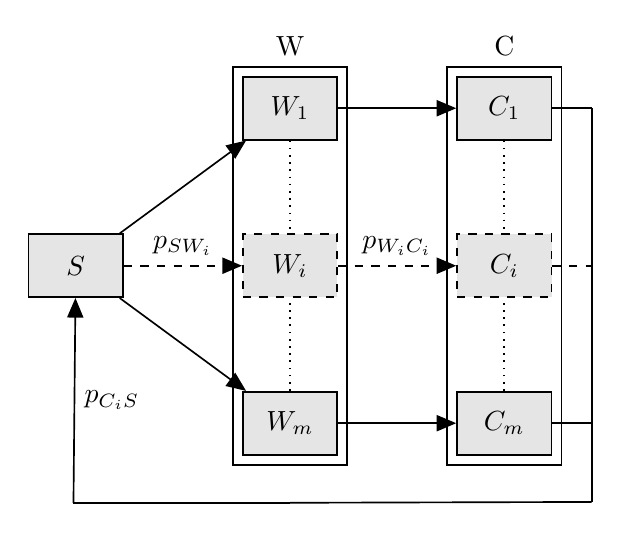
\begin{tikzpicture}[->,>=triangle 45,auto,node distance=2cm, semithick,
		state node/.style={rectangle, draw, fill=black!10, minimum height=.8cm, minimum width=1.2cm},
		meta node/.style={rectangle, draw},
		dashed node/.style={rectangle, draw, dashed, fill=black!10, minimum height=.8cm, minimum width=1.2cm}]

 	\node[state node] (1) {$S$};
 	\node[dashed node] (2) [right = 1.5cm of 1] {$W_i$};
 	\node[state node] (3) [above of=2] {$W_1$};
 	\node[state node] (4) [below of=2] {$W_m$};
 	\node[meta node, fit={(2) (3) (4)},label=above:{W}] {};
 	\node[dashed node] (5) [right = 1.5cm of 2] {$C_i$};
 	\node[state node] (6) [above of=5] {$C_1$};
 	\node[state node] (7) [below of=5] {$C_m$};
 	\node[meta node, fit={(5) (6) (7)}, label=above:{C}] {};
 	\coordinate[right=0.5cm of 6] (8);
 	\coordinate[right=0.5cm of 6] (8);
 	\coordinate[right=0.5cm of 6] (8);
 	\coordinate[right=0.5cm of 6] (8); 	 	
 	\coordinate[below of=8] (9);
 	\coordinate[below of=9] (10);
 	\coordinate[below= 1cm of 10] (11); 
 	\coordinate[below= 0.6cm of 4] (12);
 	\coordinate[left= 2.75cm of 12] (13);

		\path	(1) 	edge[dashed] node{$p_{SW_i}$} (2)
						edge[] node{} (3)
						edge[] node{} (4);
		\path	(2) 	edge[dashed] node{$p_{W_iC_i}$} (5);
		\path	(3) 	edge[] node{} (6)
						edge[-,dotted] node{} (2);		
		\path	(4) 	edge[] node{} (7)
						edge[-,dotted] node{} (2);		
		\path	(5) 	edge[-, dashed] node{} (9);
		\path	(6) 	edge[-] node{} (8)
						edge[-, dotted] node{} (5);
		\path	(7) 	edge[-, dotted] node{} (5)		
						edge[-] node{} (10);		
		\path	(8) 	edge[-] node{} (9);
		\path	(9) 	edge[-] node{} (10);
		\path	(10) 	edge[-] node{} (11);
		\path	(11) 	edge[-] node{} (12);
		\path	(12) 	edge[-] node{} (13);
		\path	(13) 	edge[] node[right= 0cm of 13]{$p_{C_iS}$} (1);
\end{tikzpicture}
\caption{Agent controller used to drive group collaboration. There is a Search state and $m$ Wait and Collaboration states, $W_i$ and $C_i$ respectively---one for each collaboration site.}\label{fig:sm}
\end{figure}

In order to compare the dynamics of the proposed probabilistic task allocation mechanism with the deterministic one by Lerman et. al\cite{Lerman2001}, we implemented a variation of the above algorithm using a unit-step at $\tau$ instead of the sigmoid function and removing the consensus step, which is not necessary in this model. 

We use Gillespie simulation \cite{gillespie76} to explore the dynamics of the proposed collaboration model.
Table~\ref{tab:params} lists the common system parameters used for all experiments. For both experiments a single collaboration site is used and each run simulates 300s of time. The desired group size ($\tau$, in Eq.~\eqref{eq:sig}) is set to 4, 8, 16 and 32 agents. The collaboration task is programmed to take 10s, on average, per agent. Data points are gathered by averaging data from 100 identically set up runs in each case. The \emph{rate of collaboration} for the threshold model is computed by summing the number of groups that successfully collaborate and dividing by the total experiment time (300s). For the deterministic model, collaboration rate is computed by summing all successful collaborations, i.e. collaborations involving team sizes equal to $\tau$, and dividing the the experiment time (300s).

\rowcolors{1}{lightgray}{white}
\begin{table}
\centering\begin{tabular}{|c|c|c|}
\hline
\# Agents & Arena Area & Area per Site\\
100 & $100cm^2$ & $10cm^2$\\
\hline
\end{tabular}
\centering\caption{}\label{tab:params}
\end{table}



%%%%%%%%%%%%%%%%%%%%%%%%%%%%%%%%%%%%%%%%%%%%%%%%%%%%%%%%%%%%%%%%%%%%%%%%%%%%%%%%
\section{Results}
\begin{figure*}[!htb]
\begin{subfigure}{0.33\textwidth}
\centering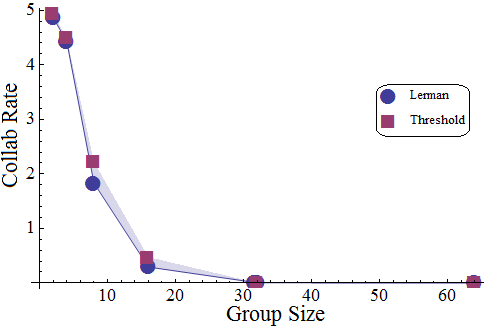
\includegraphics[width=4.5cm]{figures/LermanCollabCompare3.png}
\centering\caption{$\theta=2$}\label{fig:lercol3}
\end{subfigure}~
\begin{subfigure}{0.33\textwidth}
\centering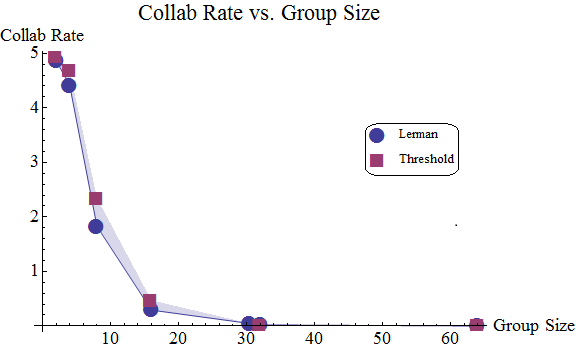
\includegraphics[width=4.5cm]{figures/LermanCollabCompare2.png}
\centering\caption{$\theta=1$}\label{fig:lercol2}
\end{subfigure}~
\begin{subfigure}{0.33\textwidth}
\centering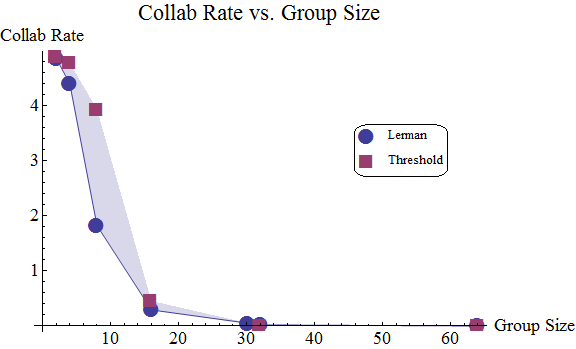
\includegraphics[width=4.5cm]{figures/LermanCollabCompare1.png}
\centering\caption{$\theta=0$}\label{fig:lercol1}
\end{subfigure}
\caption{Comparison of the collaboration rate for task allocation with probabilistic and deterministic \cite{Lerman2001} for different values of $\theta$ and team sizes $\tau$ in an environment with one collaboration site and one hundred robots. }\label{fig:lercol}
\end{figure*}

We will first compare the dynamics of the proposed approach with Lerman et al.'s k-collaboration model \cite{Lerman2001} and then validate the emergence of group sizes with similar means but varying variances.

Figure \ref{fig:lercol1} shows collaboration rates for both models when $\theta$ is set to 2 (for the probabilistic model) and the wait time is set to $\infty$ (for the deterministic model), in order to allow for a fair comparison. (All experiments are run in an regime where infinite wait times are optimal wait times in \cite{Lerman2001}.) Figures \ref{fig:lercol3}, \ref{fig:lercol2} and \ref{fig:lercol1} show collaborations rates for $\theta = 2$, $\theta = 1$ and $\theta=0$ with infinite wait time. With $\theta=0$, the logistic function is uniformly 0.5, allowing any team size to form.  
With increasing $\theta$ the Logistic function approximates a unit step, minimizing the variance. 

\begin{figure*}[!htb]
\begin{subfigure}{0.5\textwidth}
\centering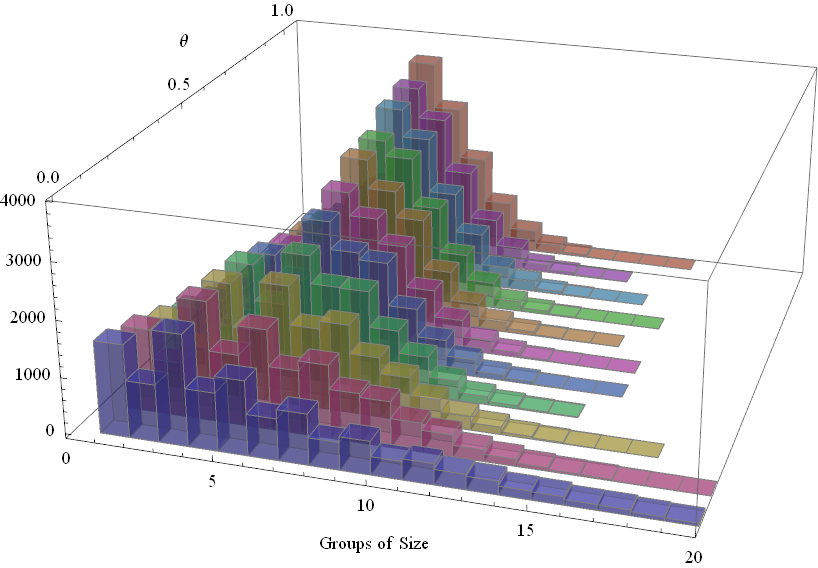
\includegraphics[width=7.5cm]{figures/collabratesweep4.png}
\centering\caption{$\tau = 4$}\label{fig:collabsweep4}
\end{subfigure}~
\begin{subfigure}{0.5\textwidth}
\centering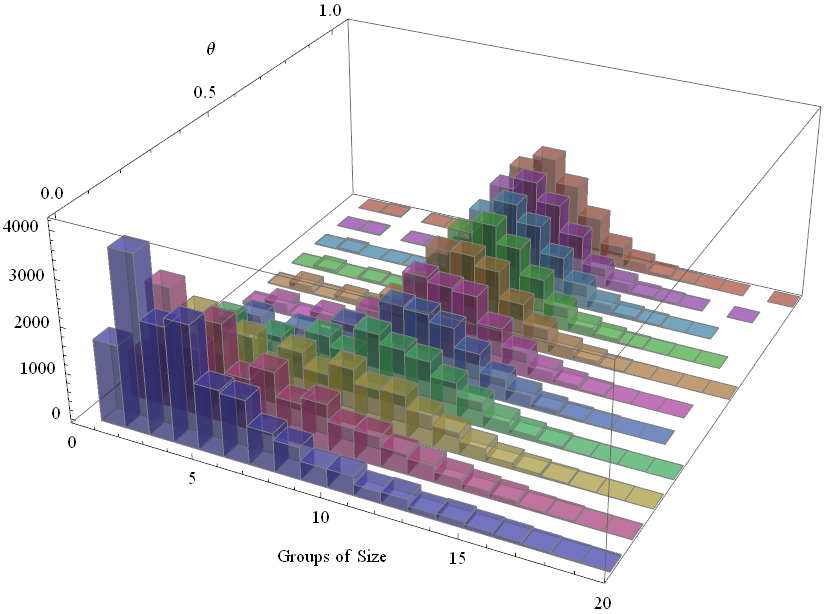
\includegraphics[width=7.5cm]{figures/collabratesweep8.png}
\centering\caption{$\tau = 8$}\label{fig:collabsweep8}
\end{subfigure}
\begin{subfigure}{0.5\textwidth}
\centering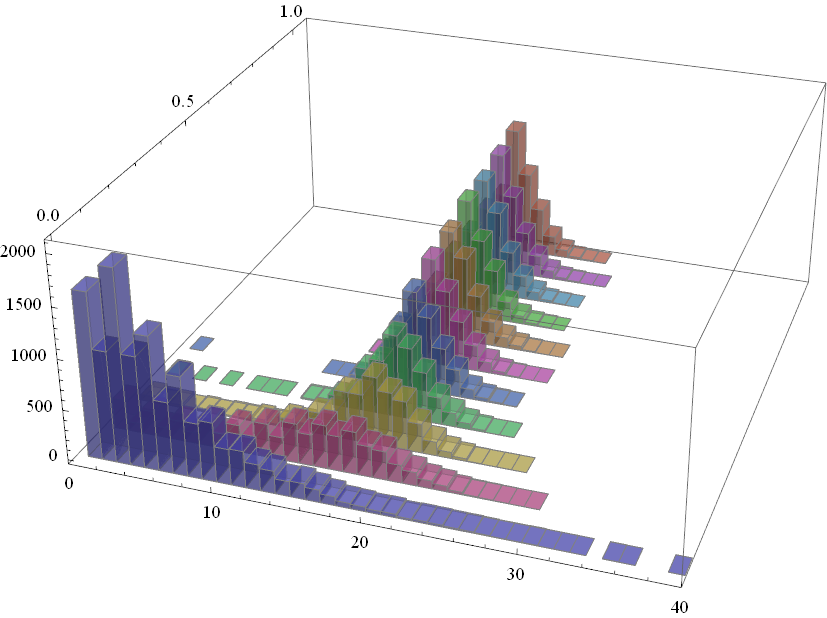
\includegraphics[width=7.5cm]{figures/collabratesweep16.png}
\centering\caption{$\tau = 16$}\label{fig:collabsweep16}
\end{subfigure}~
\begin{subfigure}{0.5\textwidth}
\centering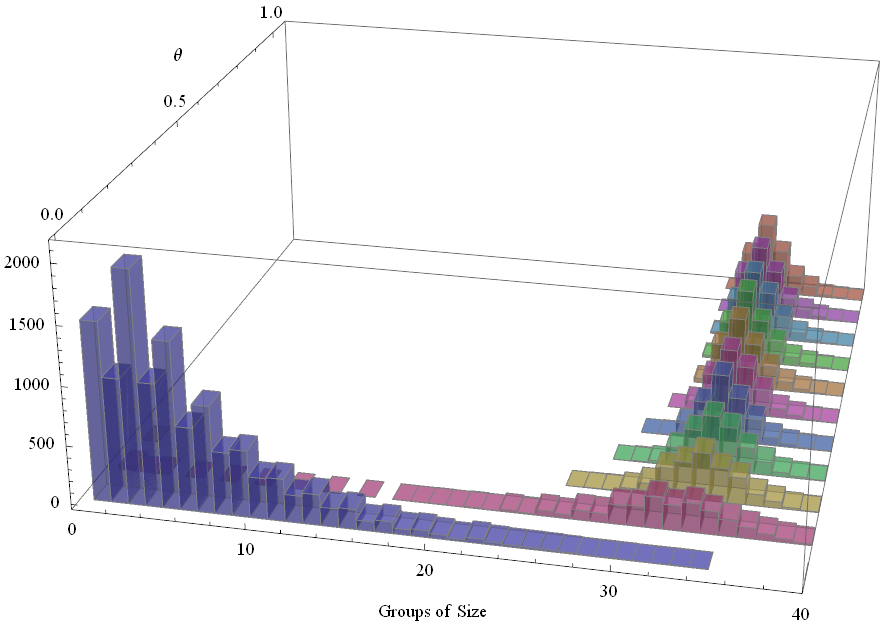
\includegraphics[width=7.5cm]{figures/collabratesweep32.png}
\centering\caption{$\tau = 32$}\label{fig:collabsweep32}
\end{subfigure}
\caption{Histograms of resulting team sizes for various values of $\tau$ and $\theta$ with one hundred robots and one collaboration site.}\label{fig:collabsweep}
\end{figure*}

We observe the collaboration rate to be qualitatively and quantitatively very similar for high values of $\theta$ (steep slope), and to exceed that of the deterministic model for very low values of $\theta$ (flat slope). This is expected as flat slopes increase the variance of the observed group size and therefore allow much smaller teams than $\tau$ agents to collaborate.

\begin{figure*}[!htb]
\begin{subfigure}{0.5\textwidth}
\centering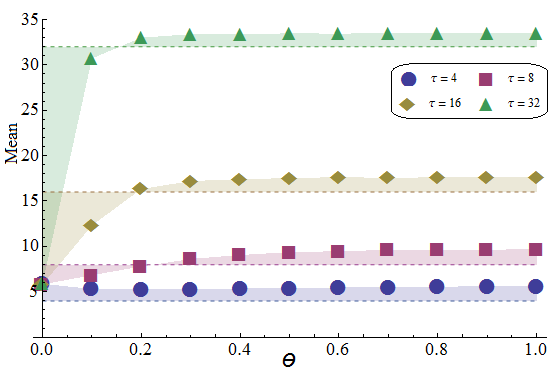
\includegraphics[width=7.5cm]{figures/means.png}
\centering\caption{}\label{fig:means}
\end{subfigure}~
\begin{subfigure}{0.5\textwidth}
\centering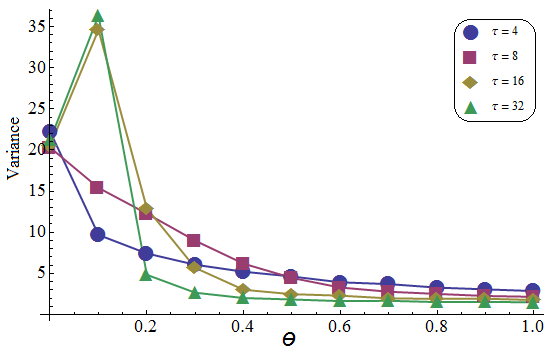
\includegraphics[width=7.5cm]{figures/variances.png}
\centering\caption{}\label{fig:vars}
\end{subfigure}
\caption{Showing the effects of varying $\theta$ on means and variances corresponding to the histograms seen in Fig.~\ref{fig:collabsweep}.}\label{fig:meansvars}
\end{figure*}

Figure \ref{fig:collabsweep} shows histograms of the resulting group sizes for various values of $\tau=4, 8, 16, 32$ and $\theta=[0;0.1;1]$ (100 simulations per data point). It is clearly seen that when $\theta$ is set to 0, the sigmoid becomes constant ($\sig(x) = 1/(1 + e^{0}) = 0.5$) so agents have an equal probability to want to collaborate or not, no matter what the desired group size is. We therefore see a large number of small groups forming, with most groups consisting of 2 agents. This is to be expected since the expected number of agents willing to collaborate in a group of size 2 is 1, given the probability of collaboration is constant at 0.5.

Figure \ref{fig:means} displays average group sizes as $\theta$ is varied from 0 to 1 and $\tau$ from 4 to 32 based on the data from Figure \ref{fig:collabsweep}. We observe that for large enough values of $\theta$ the mean of the group size distribution approaches the desired group size and is largely unaffected by increasing $\theta$. Thereafter, its magnitude depends only on $\tau$ except in the special case where $\theta = 0$ where it is constant. The relative error of the mean compared to the desired average decreases with increasing number of agents as the  Binomial distribution \eqref{eq:cdf}
approximates the Normal distribution \eqref{eq:normalcdf}.

Figure \ref{fig:vars} shows how the variance of group size decreases with increasing $\theta$. This is because the sigmoid function approximates the unit step, making the team size more and more deterministic. On the other hand, low values of $\theta$ lead to large variances in the group size. For $\theta=0$, the variance is constant for all values of $\tau$ and depends exclusively on the total number of robots. 




%Both these plots in 


%%%%%%%%%%%%%%%%%%%%%%%%%%%%%%%%%%%%%%%%%%%%%%%%%%%%%%%%%%%%%%%%%%%%%%%%%%%%%%%%
\section{Discussion}\label{sec:discussion}
Results in Figures \ref{fig:lercol}, \ref{fig:collabsweep} and \ref{fig:meansvars} show that the proposed threshold-based task allocation mechanism is a generalization of the deterministic Lerman model in that it allows to approach what is seen with deterministic group sizes while retaining the elasticity to vary group sizes along any desired range of values. Also, these plots show how altering microscopic control parameters within the agents, $\theta$ and $\tau$ of their sigmoid functions, directly affects macroscopic behavior of the swarm system by altering means and variances of formed group sizes, respectively. Although the matching between microscopic results and macroscopic prediction is not perfect due to the discrete approximation, the plots show that a wide range of means and variances are feasible. Finding appropriate parameters to reach these could be easily achieved using a suitable optimization framework such as presented in \cite{Correll2008,Berman2009}, using the macroscopic predictions as initial estimate. 

The proposed task allocation algorithm requires an estimate of the group size at each collaboration site as well as the ability to communicate with the group in order to reach a consensus. While these assumptions seem to be limiting at first sight, they can be rolled into the analysis process and possibly exploited to design the task allocation process. For example, an increasing variance for observing the group size $\tau$ or noise in the consensus process simply increase the variance of the task allocation process and could therefore be countered---to some extent---by altering the properties of the response threshold function. 

Although the algorithm does not deadlock---the probability to collaborate even if the team size is far off the desired value---the resulting behavior might be undesirable, resulting in potentially very long wait times and poor task performance. This could be mitigated by introducing preferential detachment from small groups and preferential attachment to larger groups as customary in swarm robotic aggregation \cite{correll2011modeling}.

In practice, effective collaboration rates will also be limited by the embodiment of the robots, which might finding physical space at a site cumbersome. In the presented microscopic simulation, for both stochastic and deterministic team sizes, the number of robots per site were not limited, allowing scenarios in which multiple groups collaborate in quick succession at the same site. While comparing both models without embodiment is reasonable, we wish to study the effect of embodiment in future work.

%%%%%%%%%%%%%%%%%%%%%%%%%%%%%%%%%%%%%%%%%%%%%%%%%%%%%%%%%%%%%%%%%%%%%%%%%%%%%%%%
\section{Conclusion}\label{sec:conclusion}
This paper introduces a task allocation algorithm that allows to recruit an approximate number of agents with a desired variance to a task. This allows to trade-off task execution accuracy with speed, resulting in increasing collaboration rates for teams with larger variances. 
We demonstrate that task allocation of teams with deterministic size is a subset of the proposed stochastic task allocation mechanism. As such, the proposed framework provides a computationally simple, adaptive, and robust alternative for coordination.

We investigate the limitations of the proposed approach, which shows lesser fidelity in macroscopic predictions if team sizes are small. In future work, we wish to investigate the impact of variance in estimating the number of agents waiting at a collaboration site as well as the impact of unreliable communication between agents, both of which we conjecture to impact the variance of resulting team sizes in a similar way as the slope of the response threshold function. We are also interested in studying preferential attachment/detachment techniques from swarm robotic aggregation in order to improve scenarios with insufficient numbers of robots for strong teams to emerge. 



%%%%%%%%%%%%%%%%%%%%%%%%%%%%%%%%%%%%%%%%%%%%%%%%%%%%%%%%%%%%%%%%%%%%%%%%%%%%%%%%
\section*{Acknowledgments}
This research has been supported by NSF grant xxxxxx. We are grateful for this support.

%%%%%%%%%%%%%%%%%%%%%%%%%%%%%%%%%%%%%%%%%%%%%%%%%%%%%%%%%%%%%%%%%%%%%%%%%%%%%%%%
%%%%%%%%%   The Bibliography, if any   %%%%%%%%%
\bibliographystyle{plain}		% or "siam", or "alpha", etc.
%\nocite{*}						% list all refs in database, cited or not
\bibliography{refworks}
\end{document}